\documentclass{beamer}
\usepackage[T1]{fontenc}
\usepackage[utf8]{inputenc}
\usepackage[spanish]{babel}
\usepackage{graphicx}
\usepackage{hyperref}
\usepackage{subcaption}
\usepackage{algorithm}
\usepackage{algorithmic}
\usepackage{datetime}

%packages customizations
\graphicspath{ {imgs/} }

%date without day.
\newdateformat{monthyeardate}{
  \monthname[\THEMONTH], \THEYEAR
}

\usetheme{Madrid}
\title[Seguridad en iOS y Android]{\Large Seguridad en iOS y Android: \\un Análisis Comparativo}
\institute[UNR]{\Large Tesina de Grado}
\author[Galuppo,R.]{\footnotesize Autor:\\ \small \textbf{Raúl Ignacio Galuppo}} %<= used the short author name [] for the footline
\newcommand{\director}{\footnotesize Director:\\ \small \emph{Dr. Carlos Luna}}
\date[\monthyeardate\today]

% re-definition of the title page
\setbeamertemplate{title page}{
\vfill
\centering
\begin{beamercolorbox}[rounded=true,shadow=true,sep=8pt,center]{title}
\inserttitle \par
\end{beamercolorbox}
\vfill
\usebeamerfont{institute}\insertinstitute \par
\vspace{1cm}
\begin{beamercolorbox}[leftskip=8cm,center,wd=0.7\textwidth]{author}
\begin{columns}[T]
\begin{column}{.49\textwidth}%
\centering
\insertauthor
\end{column}
\begin{column}{.49\textwidth}%
\centering
\director
\end{column}
\end{columns}
\vfill
\end{beamercolorbox}
\vfill
\centering
\vspace{1cm}
\monthyeardate\today\par
\vfill
}

\begin{document}
  \begin{frame}
    \titlepage
  \end{frame}
  
  \begin{frame}
    \frametitle{Contenidos}
    \tableofcontents[pausesections]
  \end{frame}
  
  \section{Introducción}
\subsection{Motivación}
\begin{frame}
 \begin{center}
  \LARGE Motivación
 \end{center}
\end{frame}
\begin{frame}
 \frametitle{Motivación}
 \begin{columns}
  \begin{column}[]{.40\textwidth}
   \begin{figure}[H]
    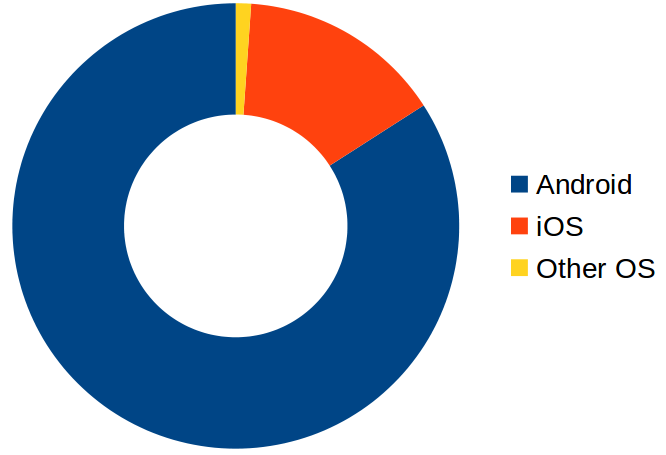
\includegraphics[scale=.15]{imgs/mobile-so-proportion.png} 
    \caption{Ventas mundiales de teléfonos inteligentes a usuarios finales por so.}
    \label{mobile-so}
   \end{figure}
  \end{column}
  \begin{column}[]{.55\textwidth}\pause
   \begin{figure}
     \centering
     \smartdiagramset{bubble node size=3.7cm,
         bubble node font=\tiny , bubble center node font=\tiny
     }
     \smartdiagram[bubble diagram]{
       Android\\más de 3.500.000,iOS\\más de 3.100.000
     }
     \caption{Cantidad de aplicaciones móviles.}
     \label{amount-apps}
   \end{figure}
  \end{column}
 \end{columns}
\end{frame}
\begin{frame}
 \frametitle{Motivación}
 \begin{exampleblock}{Motivación I}
Se incrementan los ataques a los dispositivos móviles, en busca de información personal y confidencial que almacenan, y de las operaciones realizadas a través de ellos.
  \end{exampleblock}
  \pause
  \begin{exampleblock}{Motivación II}
Debido al uso diario de estas aplicaciones, se puede filtrar una gran cantidad de información privada y confidencial.
   \end{exampleblock}
\end{frame}

\subsection{Modelo de Android}
\begin{frame}
 \begin{center}
  \LARGE Modelo de Android
 \end{center}
\end{frame}
\begin{frame}
 \frametitle{Modelo de Android}
 {Android es un sistema operativo de código abierto, diseñado para dispositivos móviles y desarrollado por Google junto con la Open Handset Alliance.}\pause
 \begin{figure}[H]
    \centering
    \begin{subfigure}{0.75\linewidth}
		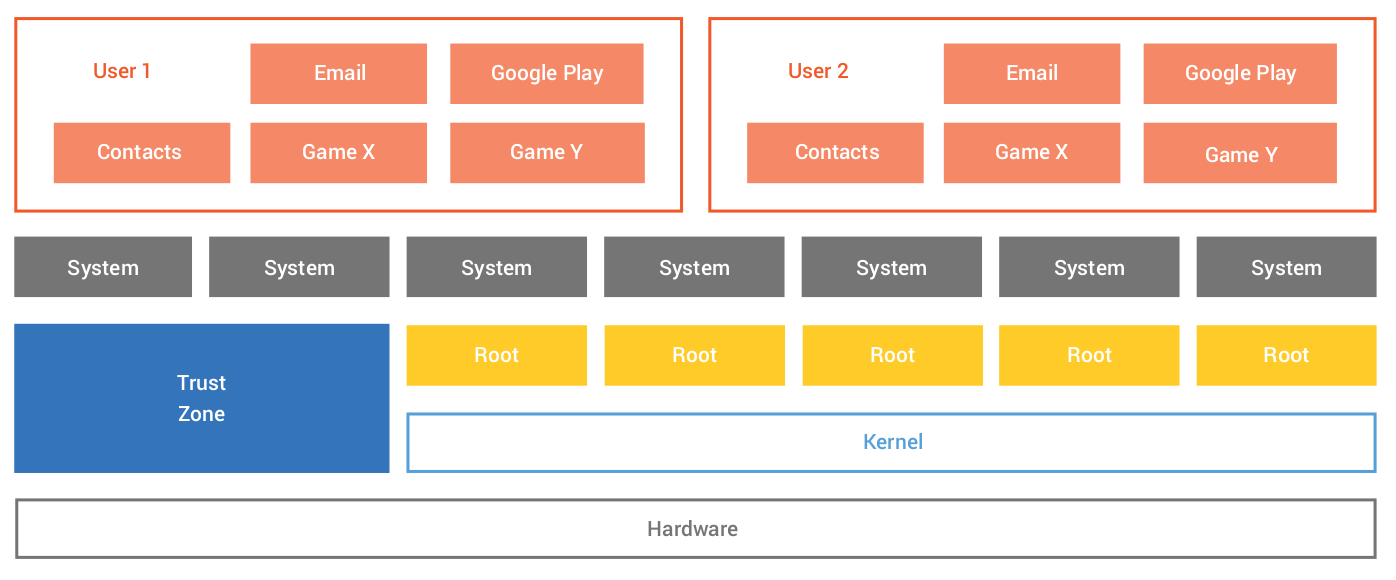
\includegraphics[width=\linewidth]{android_security_model}
	    \label{fig:ch01:sandbox}
    \end{subfigure}
    \caption{Aislamiento de las aplicaciones según su UID.}
 \end{figure}
\end{frame}
\begin{frame}
 \frametitle{Modelo de Android}
 \begin{small}
 \begin{itemize}
     \item Podemos clasificar los permisos según el riesgo implícito al otorgarlos:
     \begin{multicols}{2}
     \begin{itemize}[<+->]\small
      \item \emph{\textbf<5->{Normal}}
      \item \emph{\textbf<5->{Dangerous}}
      \item \emph{\invisible<5->{Signature}}
      \item \emph{\invisible<5->{Signature/System}}
     \end{itemize}
     \end{multicols}\pause
     \item A partir de la versión 6.0 se propone un nuevo modelo de permisos:\pause
         \begin{figure}[btp]
            \begin{subfigure}{0.4\linewidth}
            \centering
                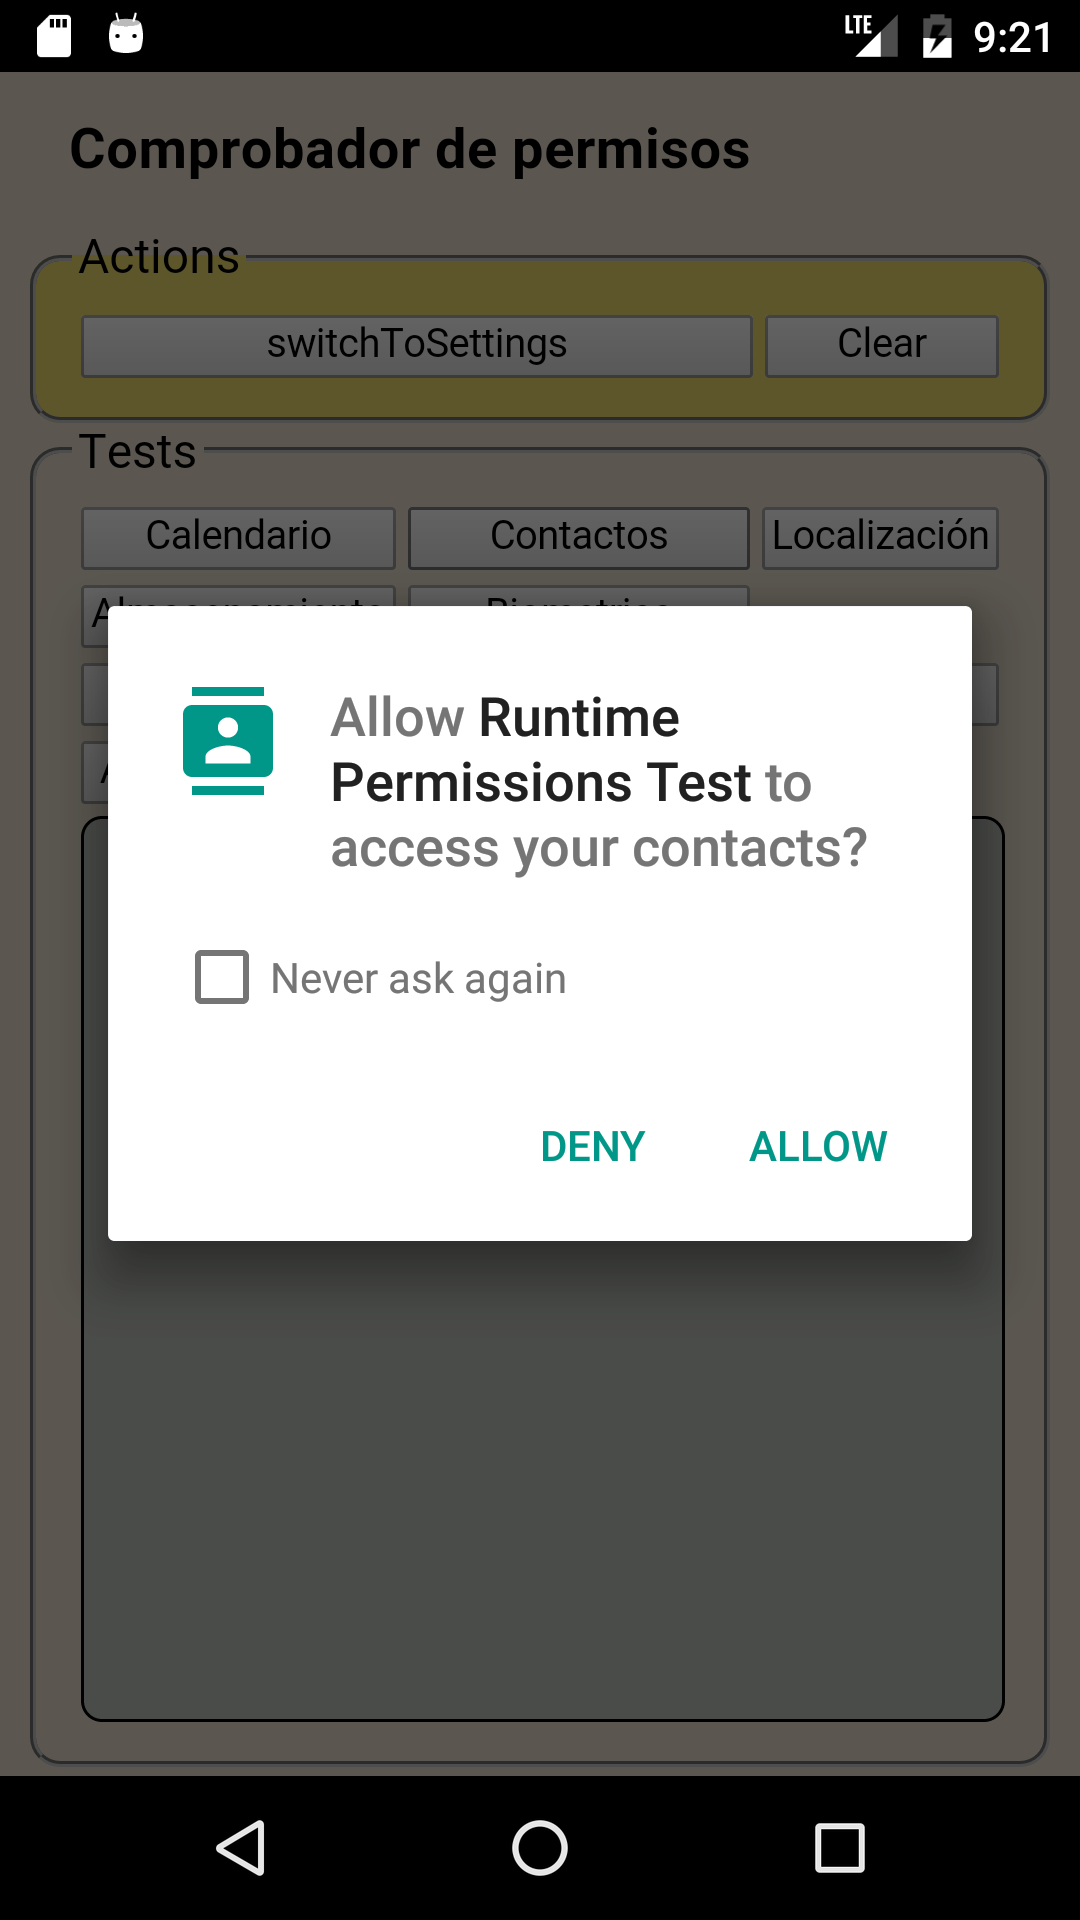
\includegraphics[width=.5\linewidth]{allow_contact}
                \caption{Solicitud de un permiso.}
            \end{subfigure}
        \begin{subfigure}{0.4\linewidth}\pause
        \centering
            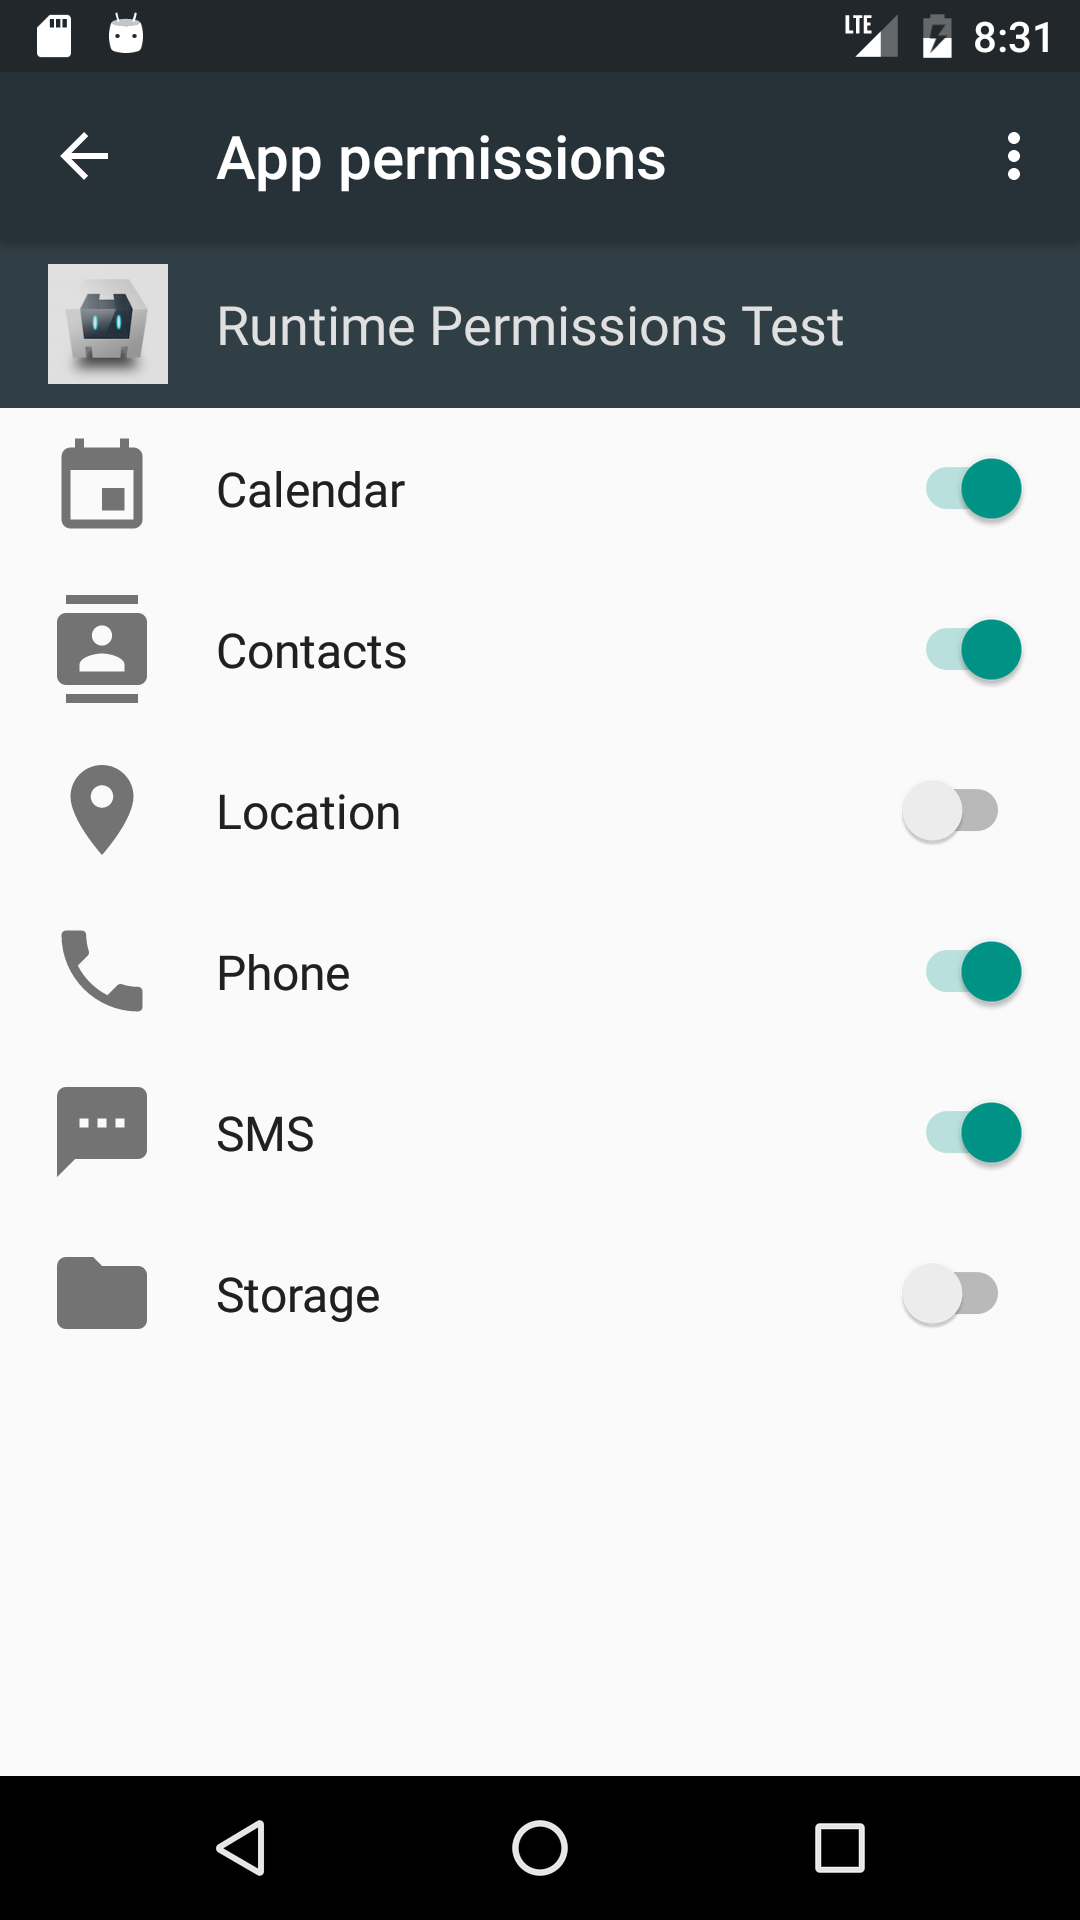
\includegraphics[width=.5\linewidth]{app-permissions}
            \caption{Listado de los permisos.}
    	\end{subfigure}
    	\caption{Nuevo modelo de permisos.}
        \end{figure}
 \end{itemize}
  \end{small}
\end{frame}

\subsection{Modelo de iOS}
\begin{frame}
 \begin{center}
  \LARGE Modelo de iOS
 \end{center}
\end{frame}
\begin{frame}
 \frametitle{Modelo de iOS}
 \begin{figure}[tH]
  \begin{subfigure}{0.7\linewidth}
   \begin{itemize}
    \item iOS es un sistema operativo para dispositivos móviles de la multinacional Apple Inc. diseñado para ser
seguro. \pause
    \item Las principales características de seguridad no son configurables y vienen habilitadas por defecto.
   \end{itemize}
  \end{subfigure}
  \begin{subfigure}{0.25\linewidth}\pause
    \centering
    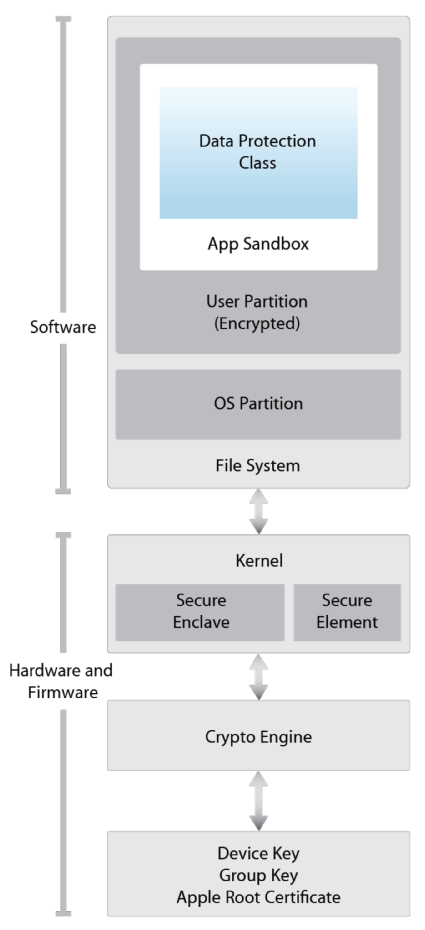
\includegraphics[width=\linewidth]{ios_security_architecture}
  \end{subfigure}
  \caption{Entorno seguro de iOS.}
\end{figure}
\end{frame}
\begin{frame}
 \frametitle{Modelo de iOS}
 \begin{itemize}
  \item Las aplicaciones pueden solicitar un permiso solamente mientras se esté ejecutando. \pause
 \end{itemize}
 \begin{figure}[hbtp]
    \centering
    \begin{subfigure}{0.49\linewidth}
    \centering
    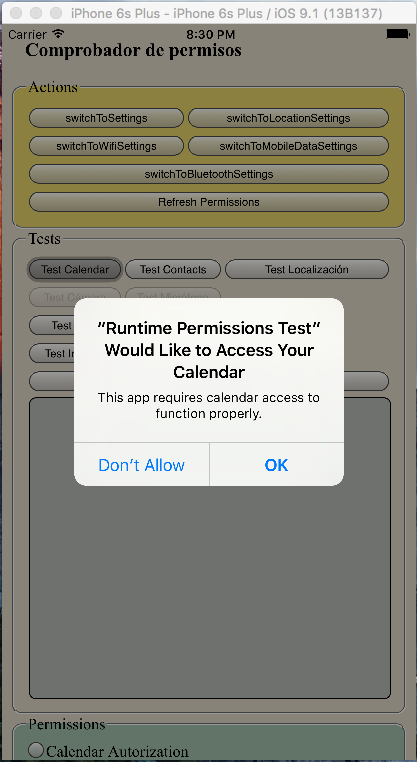
\includegraphics[width=.5\linewidth]{calendar_request_ios}
    \caption{Solicitud de un permiso.}
    \end{subfigure}
    \begin{subfigure}{0.49\linewidth}
    \centering
     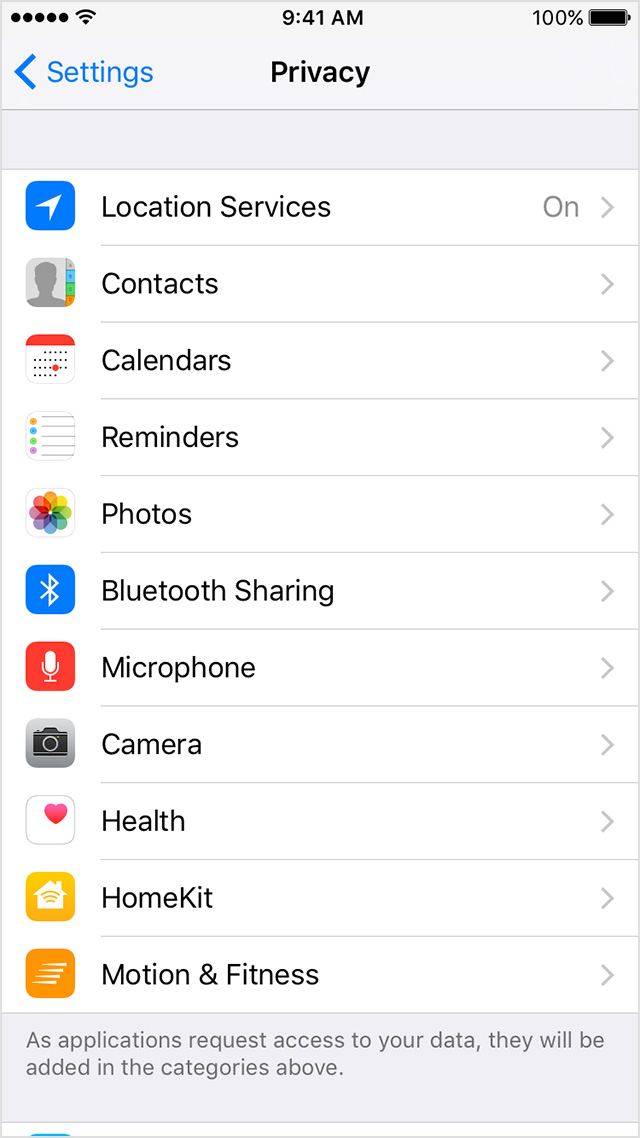
\includegraphics[width=.5\linewidth]{settings-privacy}
    \caption{Control de privacidad.}
    \end{subfigure}
    \caption{Sistema de permisos de iOS 9.}
 \end{figure}
\end{frame}


  \section{Análisis Comparativo}
\begin{frame}
 \begin{center}
  \LARGE Análisis Comparativo
 \end{center}
\end{frame}
\begin{frame}
 \frametitle{Análisis Comparativo}
 \begin{itemize}
  \item Existen muchos trabajos sobre distintas formas de comparar la seguridad de ambas plataformas.\pause
  \item Esta tesina propone analizar distintas características relacionadas a la privacidad del usuario, \pause poniendo foco en \structure{los permisos que se pueden modificar \emph{en tiempo de ejecución}}.\pause
  \item Se analizaron cuatro características presentes en iOS y Andriod:\pause
     \begin{itemize}[<+->]
      \item Arranque verificado
      \item Cifrado del sistema de archivos
      \item Bloqueo del dispositivo
      \item Seguridad de las aplicaciones
     \end{itemize}
 \end{itemize}
\end{frame}
\begin{frame}
 \frametitle{Análisis Comparativo}
Se pone foco especialmente en los sistemas de permisos:\pause
 \begin{figure}[btp]
    \centering
    \begin{subfigure}{0.23\linewidth}
        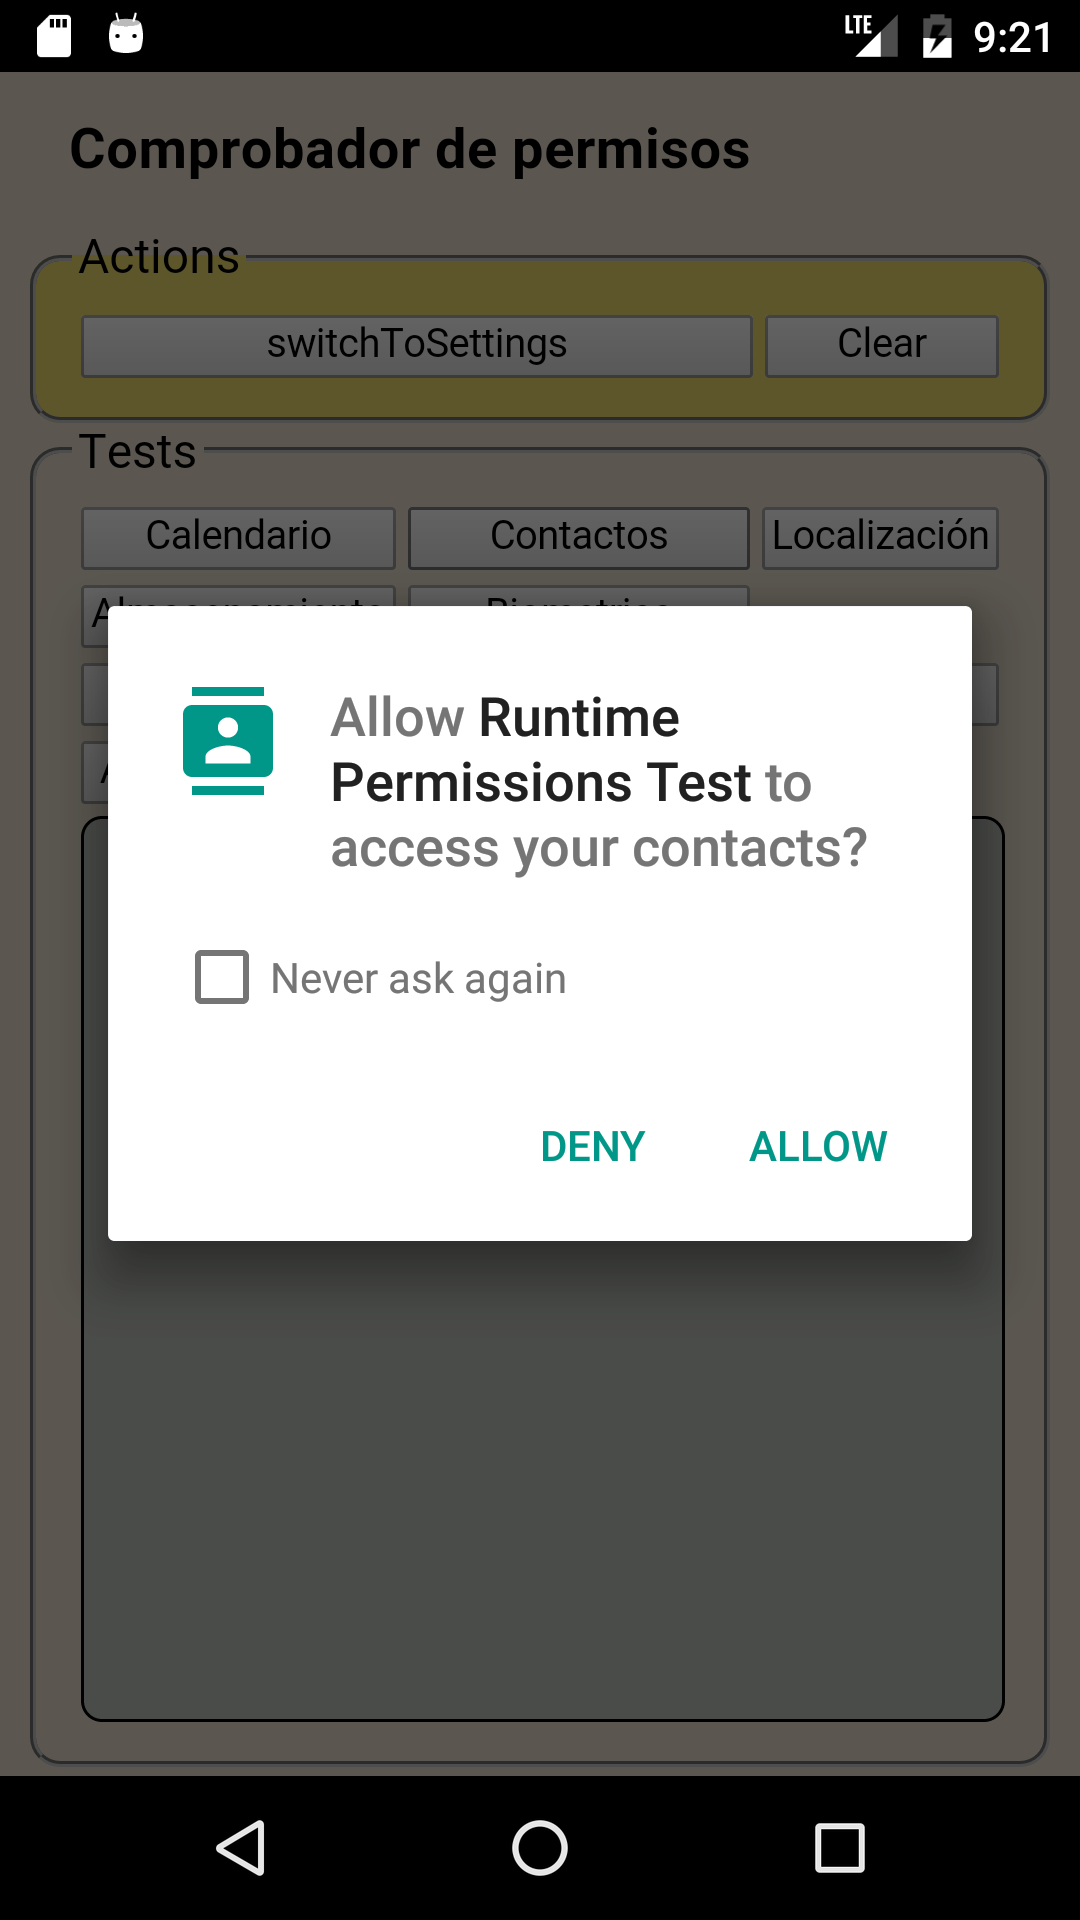
\includegraphics[width=\linewidth]{allow_contact}
        \caption{Pedido de un permiso en Android.}
    \end{subfigure}
    \begin{subfigure}{0.23\linewidth}
        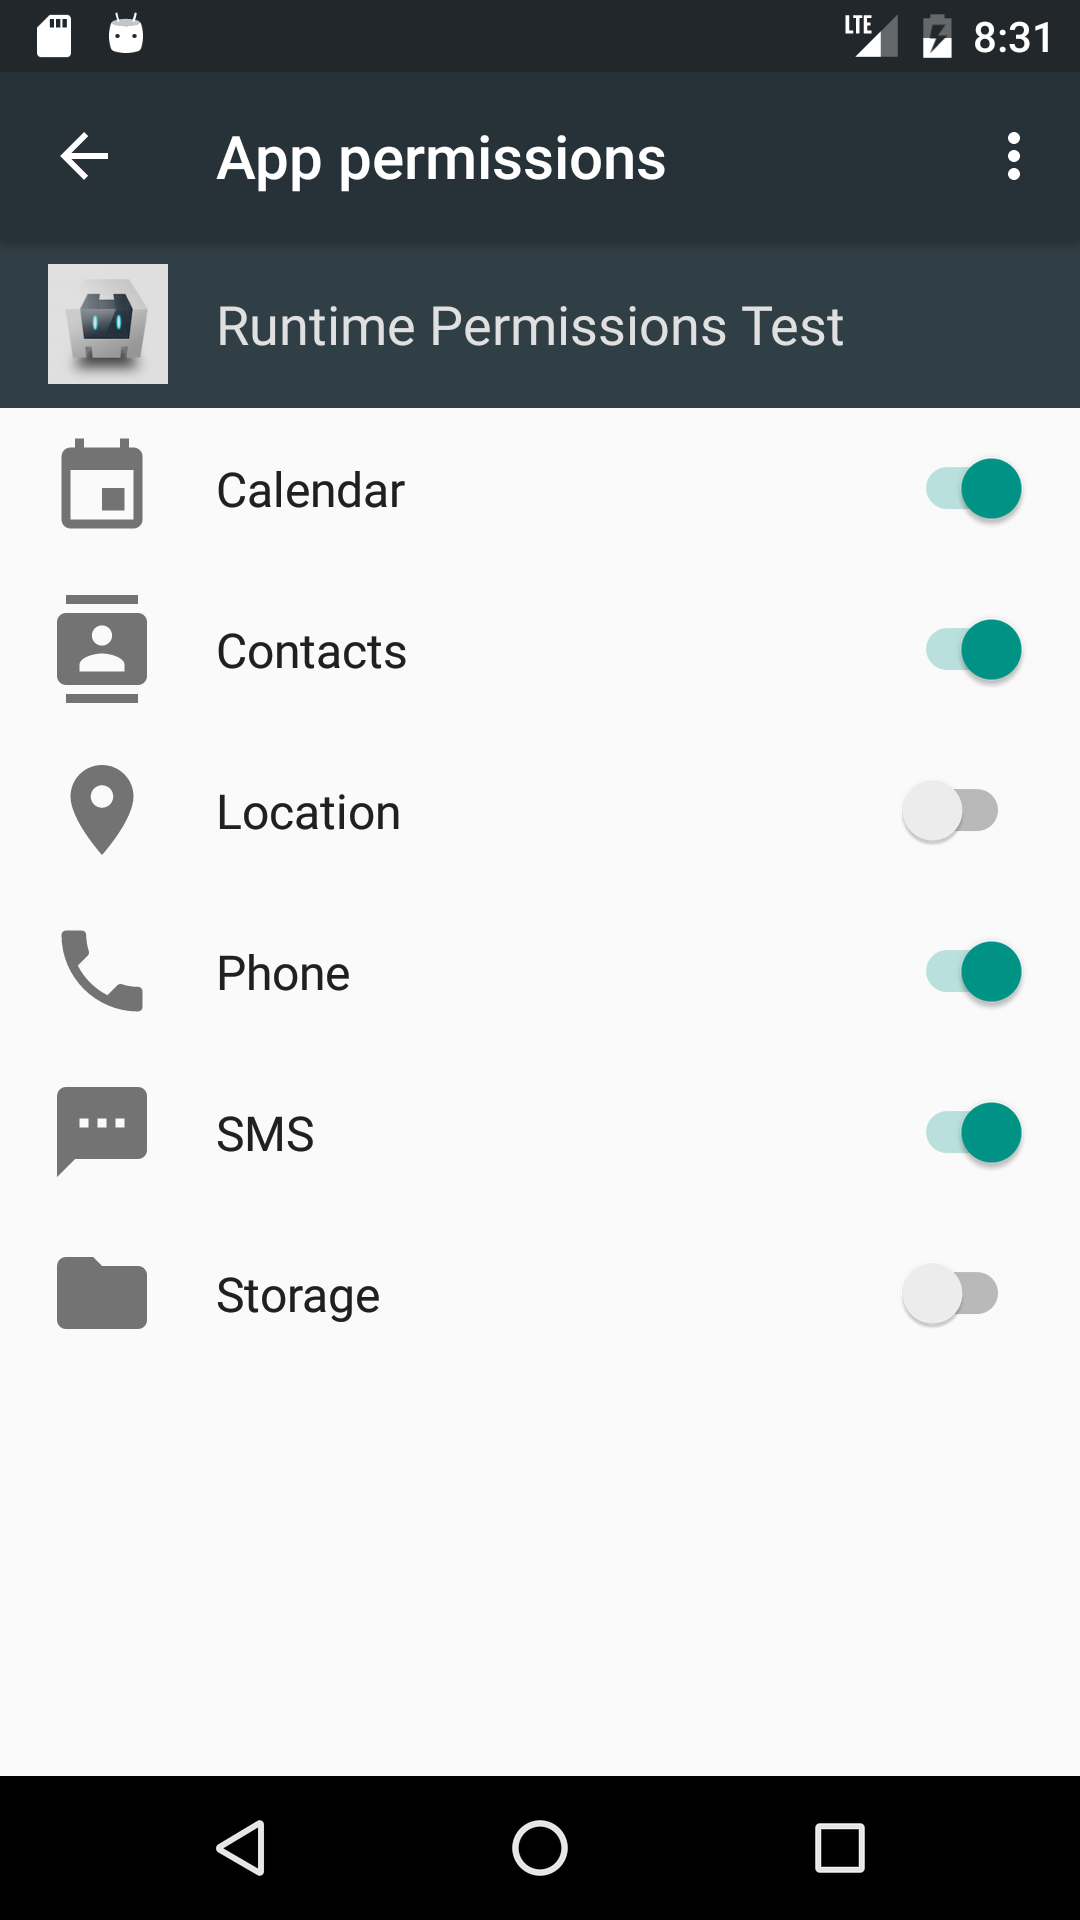
\includegraphics[width=\linewidth]{app-permissions}
        \caption{Sistema de permisos de Android.}
	\end{subfigure}\pause
	\begin{subfigure}{.23\linewidth}
    	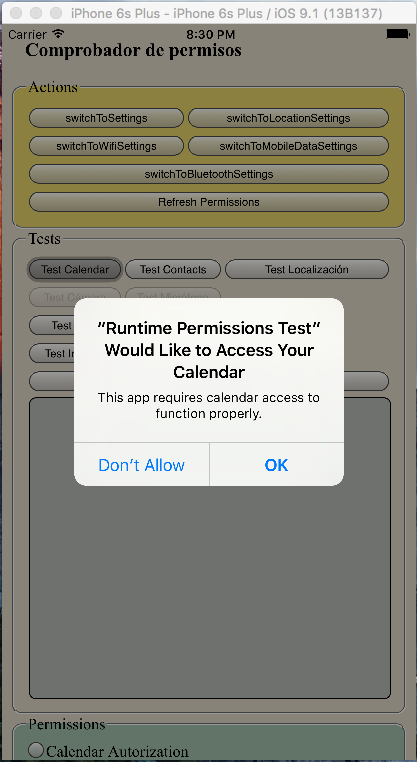
\includegraphics[width=\linewidth]{calendar_request_ios}
    	\caption{Pedido de un permiso en\\ iOS.}
    \end{subfigure}
    \begin{subfigure}{.23\linewidth}
    	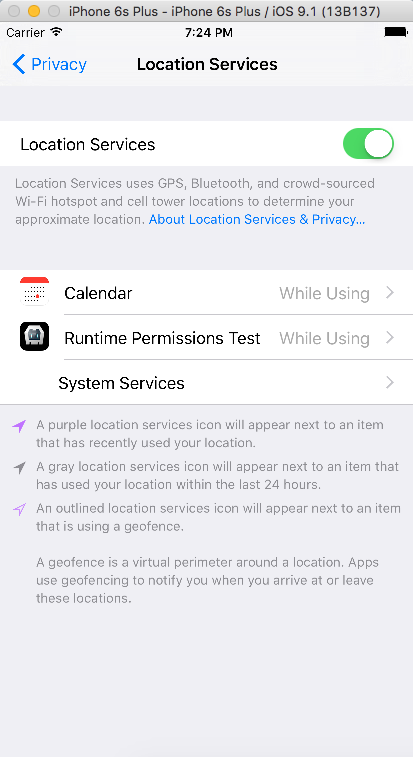
\includegraphics[width=\linewidth]{apps-allow-location}
    	\caption{Sistema de permisos de\\ iOS.}
	\end{subfigure}
	\caption{Permisos modificables en \emph{tiempo de ejecución}.}
\end{figure}
\end{frame}
\begin{frame}
 \frametitle{Análisis Comparativo}
Al comparar la gestión de permisos de ambas plataformas, encontramos varias similitudes:\pause
 \begin{itemize}[<+->]
  \item A una aplicación se le otorga permisos básicos al momento de instalación, sin posibilidad de revocarlos.
  \item Si una aplicación necesita un permiso no básico, debe requerirlo. El usuario puede otorgarlo o revocarlo.
 \end{itemize}
\end{frame}
\begin{frame}
 \frametitle{Análisis Comparativo}
Respecto a cómo se definen los permisos: \pause
 \begin{itemize}
  \item En Android están orientados según el riesgo implícito al otorgarlos.\pause
  \item En iOS los permisos están orientados a los componentes.\pause
 \end{itemize} 
  \begin{tiny}
  \begin{table}[H]
    \centering
	\begin{tabular}{c c c}
		\hline
		\multicolumn{3}{c}{\textbf{Permisos}} \\
		\emph{Ambas plataformas} 	& \emph{Solo en Android}	& \emph{Solo en iOS} \\ \hline    \hline
		Calendario	& -		& -	\\						
		Contactos	& -				& - \\						
		Cámara		& -				& -	\\						
		Localización& -				& -	\\						
		-			& -				& Compartir por Bluetooth\\ 
		Micrófono   & -				& - \\						
		-			& Teléfono		& -	\\						
		Sensores    & -    			& - \\						
		-			& SMS			& - \\						
		-			& Almacenamiento& - \\						
		-			& -				& \emph{Homekit} \\			
		-			& -				& Redes Sociales \\        	
		-			& -				& Diagnóstico \\        			
		-			& -				& Publicidad \\    			\hline
	\end{tabular}
	\caption{Resultado de la comparación de permisos.}
   \end{table}
   	\end{tiny}
\end{frame}
\begin{frame}
 \frametitle{Análisis Comparativo}
Respecto del alcance del sistema de permisos:\pause
  \begin{itemize}[<+->]
   \item En Android, un permiso es a nivel de grupo. Por lo tanto, el usuario otorga o deniega para todo el grupo.
   \item La misma situación ocurre en iOS: se otorga un permiso de acceso a todas las funcionalidades de un determinado componente.
  \end{itemize}
\end{frame}
\begin{frame}
 \frametitle{Análisis Comparativo}
Si observamos la cobertura del sistema de permisos, \pause las dos plataformas dejan funcionalidades sin permisos modificables \emph{en tiempo de ejecución}:\pause
  \begin{itemize}[<+->]
   \item En Android se destacan: Acceso a Internet, Compartir vía Bluetooth e Información del Dispositivo.
   \item En iOS se destacan: Acceso a Internet y SMS. Tampoco tiene la suficiente granularidad para administrar el acceso a los datos de las llamadas telefónicas.
  \end{itemize}
\end{frame}
\begin{frame}
 \frametitle{Análisis Comparativo}
\small {Para finalizar se analizará la interacción con el usuario:}\pause
\begin{figure}
	\centering
	\begin{subfigure}{.23\linewidth}
		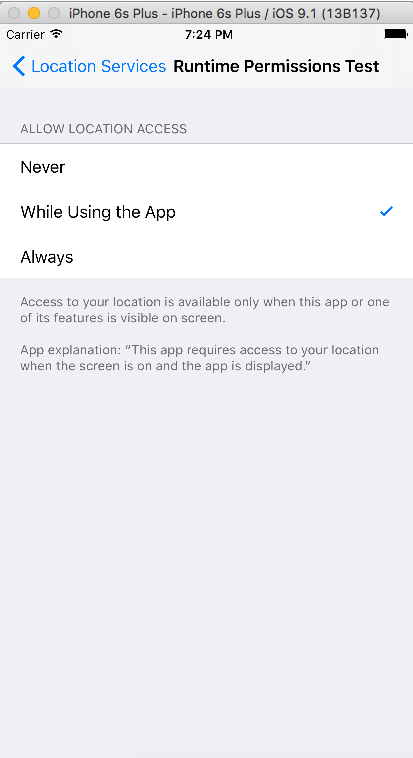
\includegraphics[width=\linewidth]{permission-classes.png}
		\caption{Permisos requeridos por una aplicación.}
		\label{fig:ch05:ios_all_permissions}
	\end{subfigure}\pause
	\begin{subfigure}{.23\linewidth}
		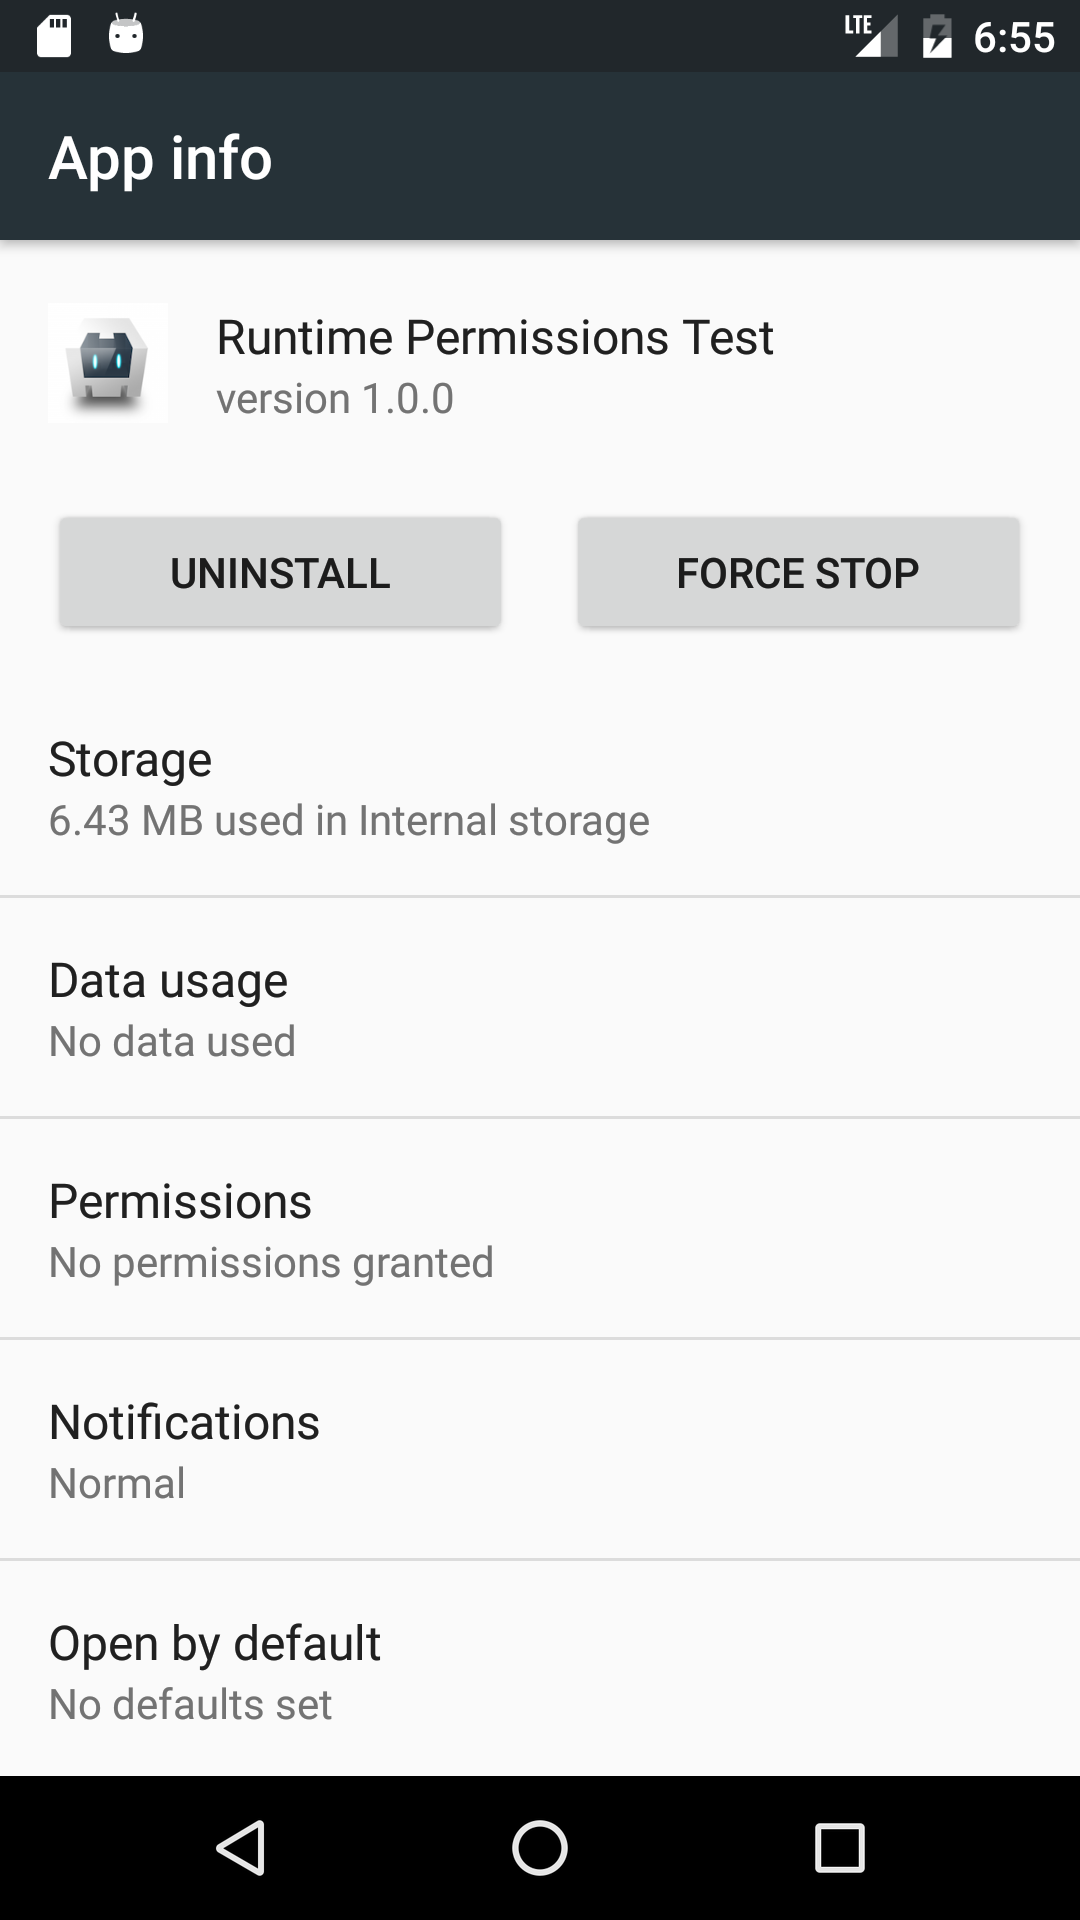
\includegraphics[width=\linewidth]{no_permissions_granted}
		\caption{La aplicación no tiene ningún permiso.}
		\label{fig:ch05:without_permissions}
	\end{subfigure}\pause
	\begin{subfigure}{.23\linewidth}
		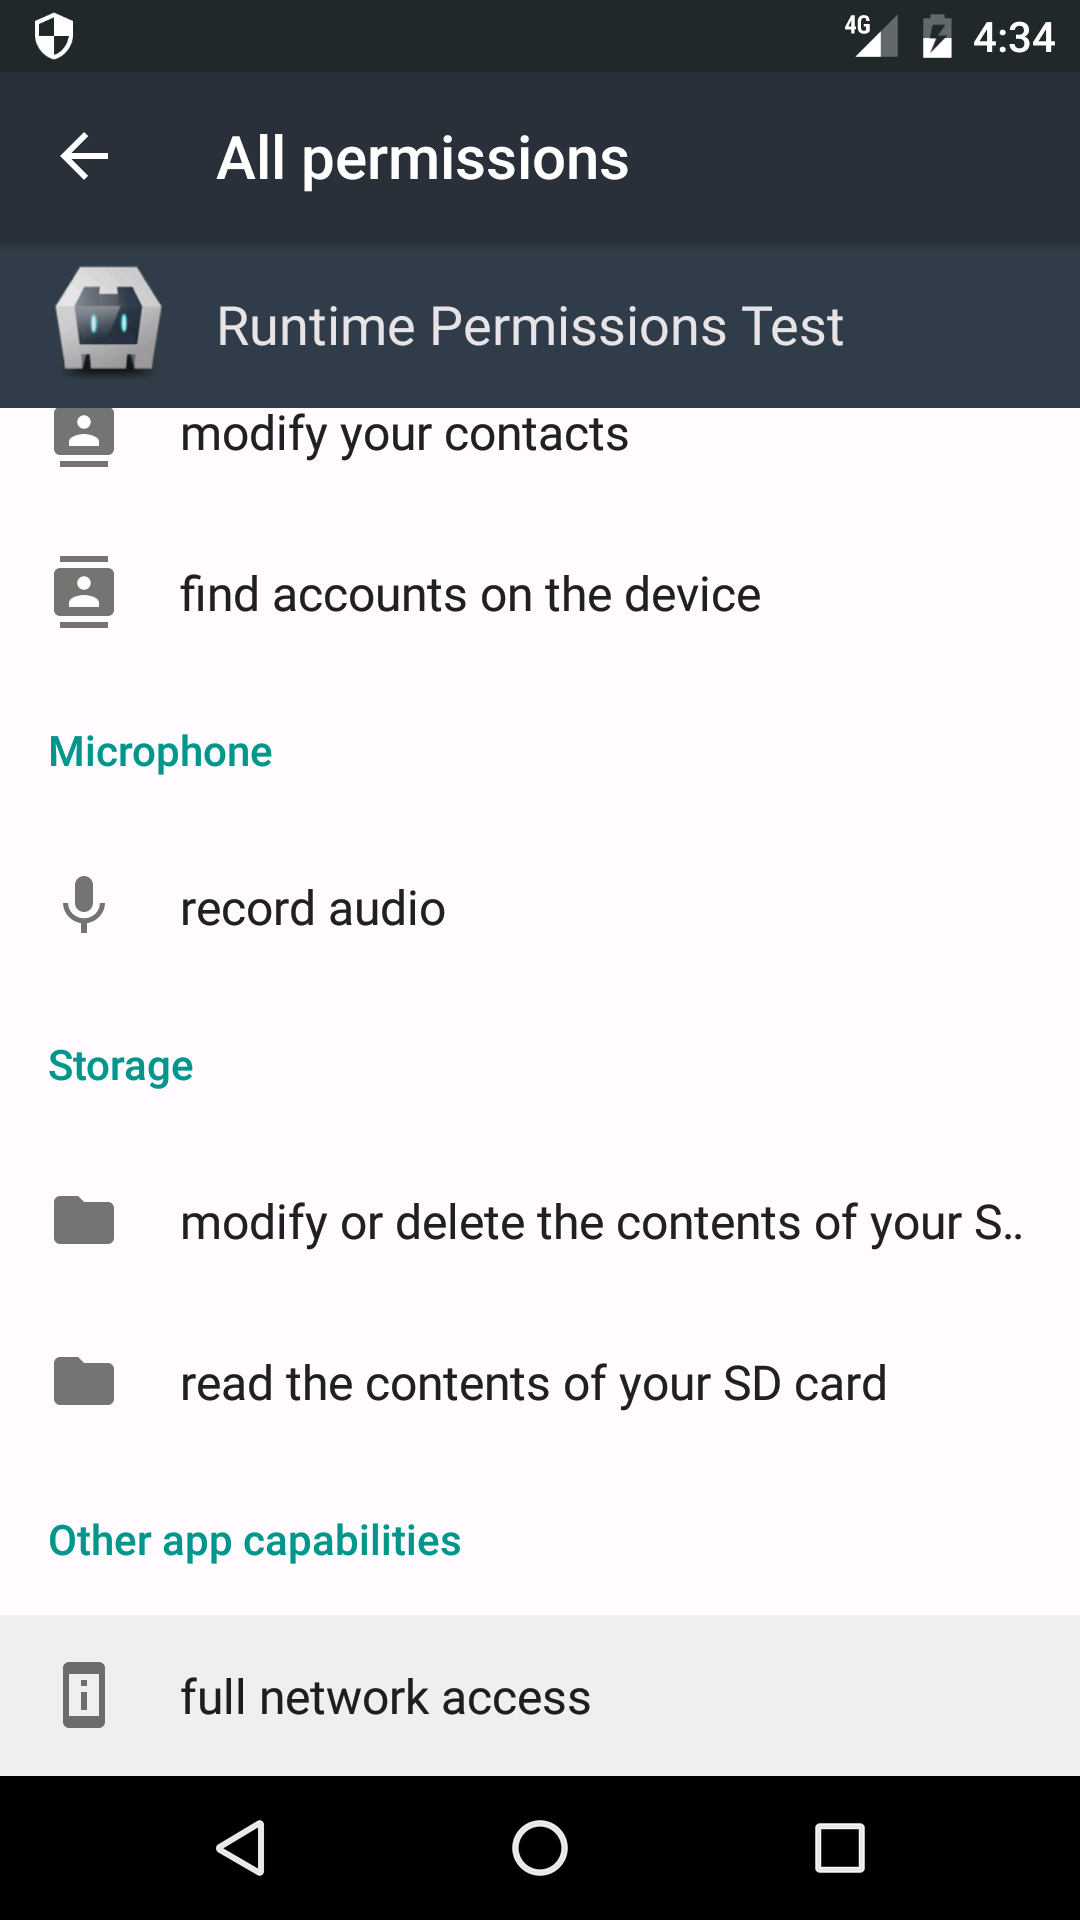
\includegraphics[width=\linewidth]{always_have_internet}
		\caption{Tiene todos los permisos \emph{normales}.}
		\label{fig:ch05:always_have_internet}
	\end{subfigure}
	\caption{Interacción con el usuario en iOS y Android.}
\end{figure}
\end{frame}
  \section{Hacia un Framework para la Comparación de Permisos}
\begin{frame}
 \begin{center}
  \LARGE Framework \\para la \\Comparación de Permisos
 \end{center}
\end{frame}
\begin{frame}
 \frametitle{Hacia un Framework para la Comparación de Permisos}
 \begin{block}{}
Se ha desarrollado un \textit{framework} para determinar empíricamente el alcance de los sistemas de permisos de ambas plataformas.
 \end{block}\pause
 \begin{columns}
  \begin{column}[]{.45\textwidth}
   \begin{exampleblock}{Objetivo I}
    {Se busca dejar en evidencia posibles vulnerabilidades presentes en los modelos de seguridad.}
   \end{exampleblock}
  \end{column}
  \begin{column}[]{.53\textwidth}\pause
   \begin{exampleblock}{Objetivo II}
    {Se intenta averiguar cuál es la cobertura del sistema de permisos respecto de los datos sensibles para la privacidad.}
   \end{exampleblock}
  \end{column}
 \end{columns}
\end{frame}
\begin{frame}
 \frametitle{Hacia un Framework para la Comparación de Permisos}
 \begin{columns}
  \begin{column}[]{.4\textwidth}
    \begin{figure}[hbtp]
     \centering
	 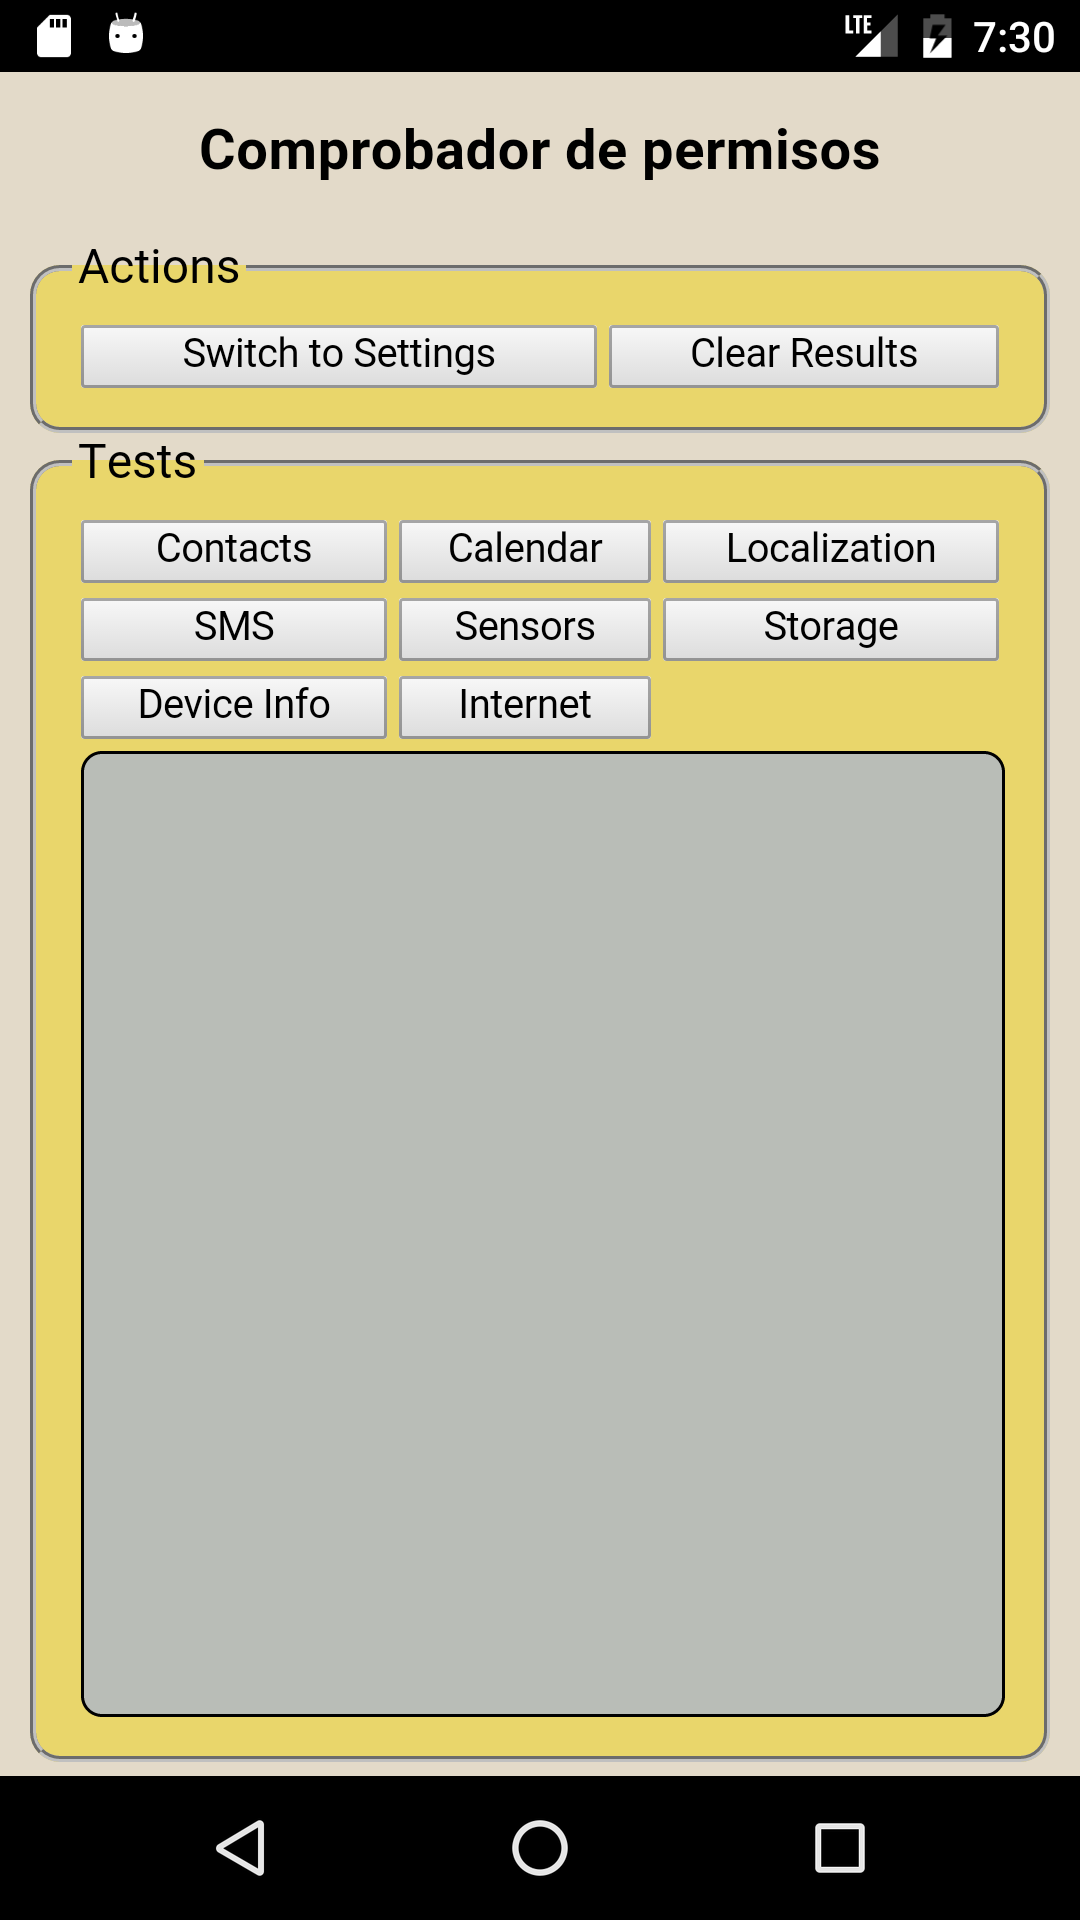
\includegraphics[width=0.75\linewidth]{app_main_view}
	 \caption{Áreas del \textit{framework}.}
	 \label{fig:chapter05:main_view}
    \end{figure}
  \end{column}
  \begin{column}[]{.58\textwidth}
  \begin{block}{}
El \textit{framework} es \alert{una aplicación móvil híbrida} \pause \structure{desarrollada con Apache Cordova} \pause y está compuesto por varios tests.
   \end{block}\pause
   \begin{block}{}
Se utilizaron los emuladores oficiales para testear el \emph{framework} propuesto.
    \end{block}
  \end{column}
 \end{columns}
\end{frame}
\begin{frame}
 \frametitle{Hacia un Framework para la Comparación de Permisos}
 \begin{columns}
  \begin{column}[]{.5\textwidth}
   Utilizando \emph{framework} se pueden testear:
   \begin{itemize}
	\item Contactos
	\item Calendario
	\item Geolocalización
	\item SMS\structure *
	\item Sensores
	\item Almacenamiento
	\item Información del dispositivo
	\item Acceso a Internet
   \end{itemize}
  \end{column}
  \pause
  \begin{column}[]{.5\textwidth}
   Sin embargo, no se pueden testear:
   \begin{itemize}
    \item \alert {WIFI}
    \item \alert {Bluetooth}
    \item \alert {NFC}
    \item \alert {Conexiones USB}
    \item \alert {Micrófono}
    \item \alert {Cámara}
   \end{itemize}
  \end{column}
 \end{columns}
\end{frame}
\begin{frame}
 \frametitle{Hacia un Framework para la Comparación de Permisos}
Por ejemplo:
\begin{figure}[hbp]
    \centering
    \begin{subfigure}{0.28\linewidth}
        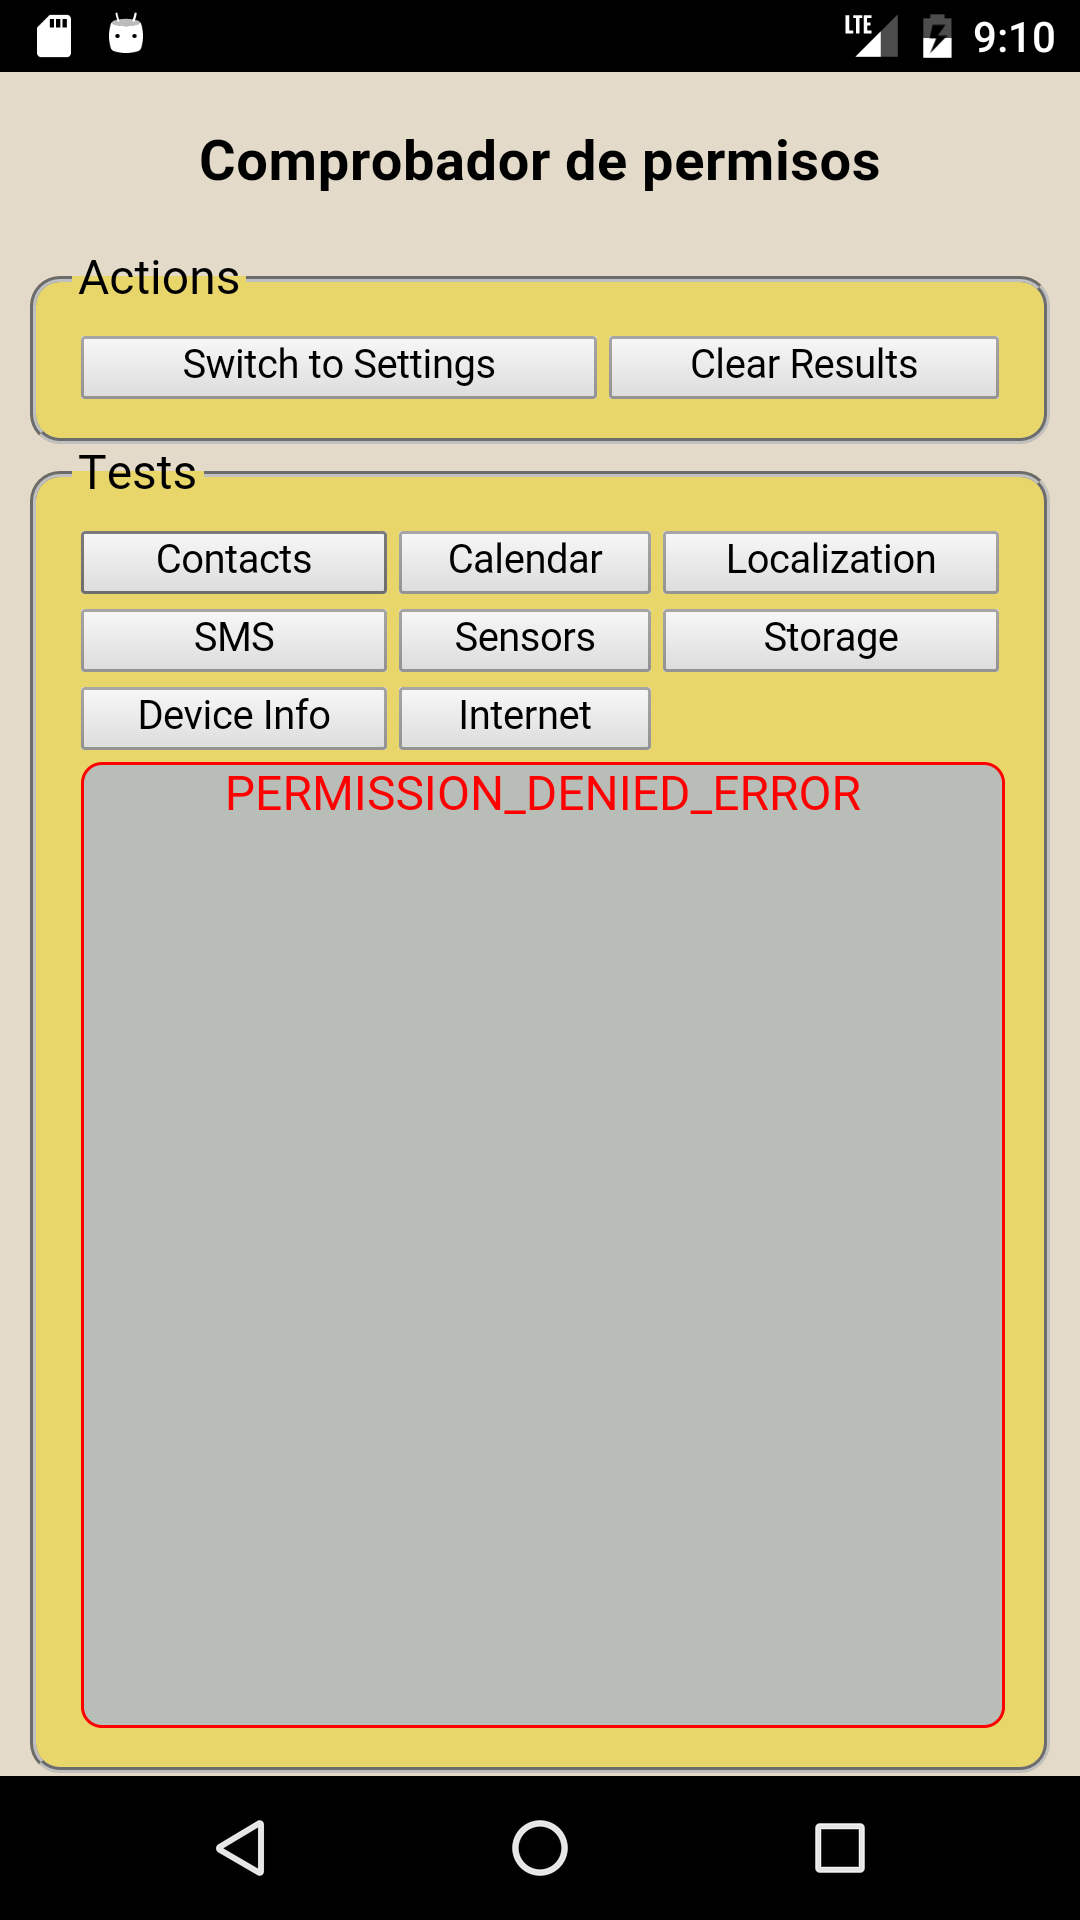
\includegraphics[width=\linewidth]{without_contact}
        \caption{Mensaje de Error.}
    \end{subfigure}
    \begin{subfigure}{0.28\linewidth}
        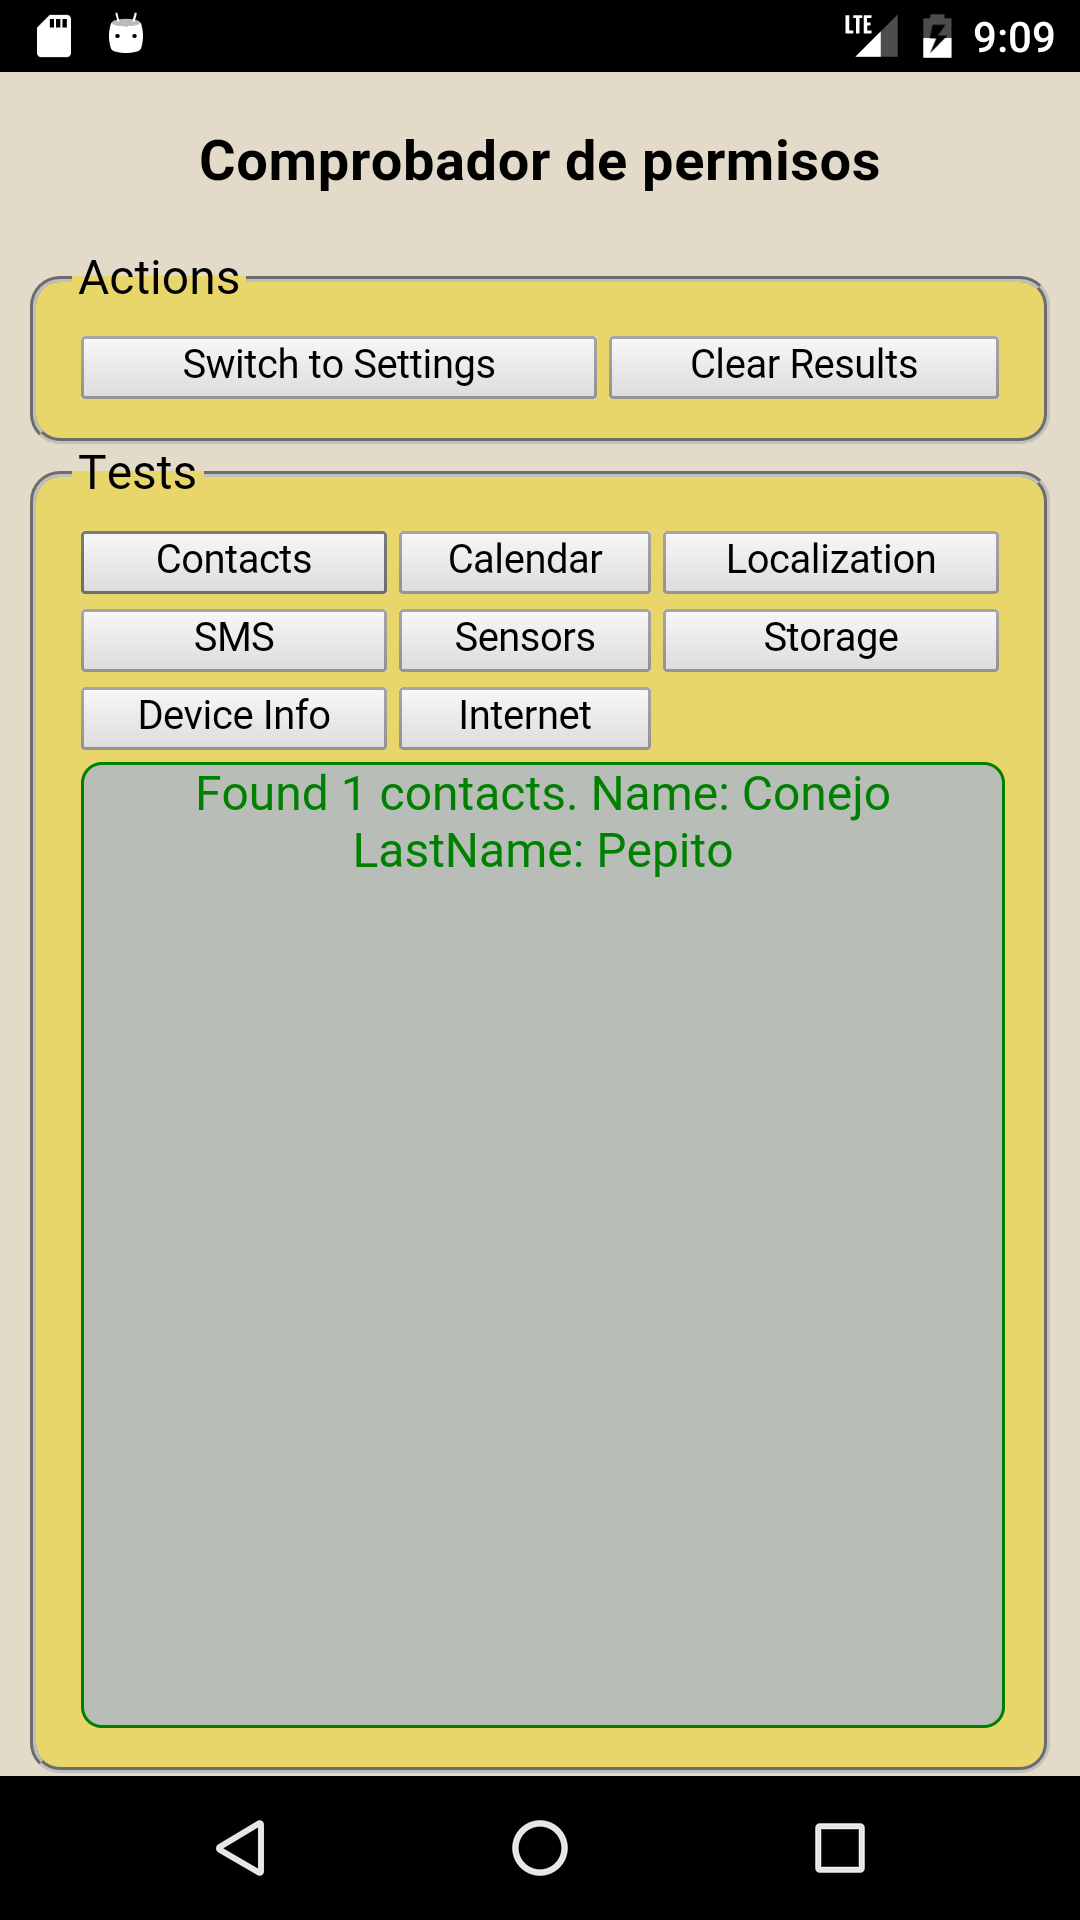
\includegraphics[width=\linewidth]{with_contact}
                \caption{Mensaje exitoso.}
     \end{subfigure}
	\begin{subfigure}{.42\linewidth}
	\begin{algorithm}[H]
	\algsetup{linenosize=\small}
    \scriptsize
	\begin{algorithmic}[1]
		\STATE Se imprimen por consola todos los contactos.
		\STATE Se crea un nuevo contacto.
		\STATE Se vuelven a imprimir por consola \\todos los contactos.
	\end{algorithmic}
	\caption{\centering Test de Contactos}
   \end{algorithm}
   \begin{block}{}\small
    {Es necesario tener el permiso \texttt{Contacto}, tanto para Android como para iOS.}
   \end{block}
   \begin{block}{}\small
 {Se utilizó el \textit{plugin} \texttt{cordova-plugin-contacts} \\(v. 2.3.1).}
   \end{block}
   \end{subfigure}
    \end{figure}
\end{frame}
\begin{frame}
Se pueden clasificar los componentes según \emph{requieran autorización del usuario para utilizarlos}:\pause
  \begin{table}[H]
    \centering
    \begin{small}
	\begin{tabular}{c c c c}
		\hline
		\multicolumn{4}{c}{\emph{\textbf{Permisos}}} \\
		\emph{Clase A} 	& \emph{Clase B}	 & \emph{Clase C}    & \emph{Clase D}\\ \hline \hline
    Contactos    & -    & -    & -\\
    Calendario    & -    & -    & -\\
    Geolocalización    & -    & -    & -\\
    -    & SMS & -    & -\\
    -    & Almacenamiento    & -    & -\\
    -    & -    & -    & Sensores\\
    -    & -    & -    & Información del dispositivo\\
    -    & -    & -    & Acceso a Internet\\ \hline
	\end{tabular}
    \caption{Clasificación de componentes.}
	\end{small}
  \end{table}\pause
  \begin{block}{}\centering
    {Dichas clases mutuamente excluyentes.}  
  \end{block}
\end{frame}
  \section{Conclusiones y Trabajos Futuros}
\begin{frame}
 \begin{center}
  \LARGE Conclusiones\\ y\\ Trabajos Futuros
 \end{center}
\end{frame}
\begin{frame}
 \frametitle{Conclusiones}
 \begin{footnotesize}
 \begin{exampleblock}{Primer Aporte}
Se realizó un análisis comparativo entre algunas características presentes en los modelos de seguridad de ambas plataformas.\\ \pause
Ellas son: verificación del arranque del sistema operativo, \pause cifrado del sistema de archivos, \pause bloqueo del dispositivo \pause y sistemas de permisos.\\ \pause
Todas ellas se eligieron porque son importantes a la hora de resguardar la privacidad del usuario.
 \end{exampleblock}\pause
 \begin{exampleblock}{\flushright {Segundo Aporte}}
Como fruto del análisis, se logró establecer una medida de comparación entre los permisos presentes en ambas plataformas. \pause La medida propuesta es la siguiente: \emph{dos permisos son similares si resguardan un componente que provee la misma funcionalidad}.\\ \pause
Utilizando la medida propuesta, todos los permisos que un usuario puede cambiar en tiempo de ejecución quedan clasificados en tres grupos: \pause \emph{Ambas Plataformas}, \pause \emph{Solo en Android} \pause o \emph{Solo en iOS}.\\ \pause
Cabe aclarar que los grupos son mutuamente excluyentes.
 \end{exampleblock}
 \end{footnotesize}
\end{frame}
\begin{frame}
 \frametitle{Conclusiones}
 \begin{footnotesize}
 \begin{exampleblock}{Tercer Aporte}
Otro aporte es el \emph{Framework para la Comparación de Permisos}. \pause Tiene dos funciones principales: \pause determinar empíricamente los alcances de los sistemas de permisos; \pause y establecer una relación entre los permisos presenten en las dos plataformas.\\ \pause
El \emph{framework} está compuesto por una batería de tests, teniendo cada uno de ellos la tarea de probar una funcionalidad provista por Android e iOS.
 \end{exampleblock} \pause
 \begin{exampleblock}{\flushright {Cuarto Aporte}}
Como resultado de la utilización del \emph{framework} se determinó una clasificación de permisos. \pause El criterio utilizado fue: \emph{un componente pertenece a una clase según requiera autorización explícita del usuario para utilizarlo}. \pause Utilizando el criterio propuesto, se obtuvieron cuatro clases mutuamente excluyentes:\pause
  \begin{scriptsize}
  \begin{itemize}[<+->]
    \item \underline{Clase A}: componentes que requieren autorización explícita en ambas plataformas para poder utilizar las funcionalidades que proveen;
    \item \underline{Clase B}: componentes que requieren autorización explícita solamente en Android;
    \item \underline{Clase C}: componentes que requieren autorización explícita solamente en iOS;
    \item \underline{Clase D}: componentes que no requieren autorización explícita para poder utilizar las funcionalidades que proveen.
  \end{itemize}
  \end{scriptsize}
 \end{exampleblock}
 \end{footnotesize}
\end{frame}
\begin{frame}
 \frametitle{Trabajos futuros}
Para finalizar, se enumeran algunas líneas a seguir como trabajos a futuro:\pause
 \begin{small}
 \begin{itemize}[<+->]
    \item Probar y mejorar los tests en dispositivos reales.
    \item Desarrollar tests para las funcionalidades que no pueden ser emuladas.
    \item Desarrollar un test para poder comparar el cifrado de archivos.
    \item No sabemos qué permisos básicos otorga iOS. Se podrían desarrollar varios tests para descubrirlos.
    \item Dado que salieron al mercado Android 8.0 e iOS 11, se podría analizar extender el \emph{framework} para las características de seguridad adicionadas en dichas versiones.
    \item En el Capítulo 4 se mencionan algunos análisis previos relacionados a la seguridad de Android y/o de iOS. Se podría profundizar más en comparar el modelo propuesto en el presente informe con los análisis mencionados previamente.
 \end{itemize}
 \end{small}
\end{frame}


  \section*{fin}
\begin{frame}
 \begin{center}
  \LARGE \textbf{¿ Preguntas ?}
  \begin{figure}[H]
    
\includegraphics[width=.4\linewidth]{preguntas}
 \end{figure}
 \end{center}
\end{frame}
\begin{frame}
 \begin{center}
  \begin{figure}[H]
    
\includegraphics[width=.5\linewidth]{deadpool-heart}
  \end{figure}
  \LARGE \textbf{¡¡ Mil gracias por venir !!}
 \end{center}
\end{frame}

\end{document}